\documentclass[11pt,letterpaper]{article}

\usepackage[margin=1in]{geometry}
\usepackage{amsmath,amssymb}
\usepackage{graphicx}
\usepackage{booktabs}
\usepackage{hyperref}
\usepackage{xcolor}
\usepackage{tikz}
\usetikzlibrary{shapes.geometric, arrows.meta, positioning, fit, backgrounds}
\usepackage{listings}
\usepackage{natbib}
\usepackage{caption}

\hypersetup{
    colorlinks=true,
    linkcolor=blue!70!black,
    citecolor=blue!70!black,
    urlcolor=blue!70!black,
}

\lstset{
    basicstyle=\small\ttfamily,
    keywordstyle=\color{blue!70!black},
    commentstyle=\color{green!50!black},
    stringstyle=\color{red!70!black},
    frame=single,
    breaklines=true,
    columns=fullflexible,
}

\title{\textbf{RubinAlerts}: A Multi-Broker Pipeline for Type~Ia Supernova\\
Discovery and Spectroscopic Follow-Up Scheduling\\
in Rubin Observatory Deep Drilling Fields}

\author{A.~Gil \and C.~Stubbs}

\date{April 2026}

\begin{document}

\maketitle

\begin{abstract}
We describe \textsc{RubinAlerts}, a two-subsystem pipeline for
discovering, prioritizing, and scheduling spectroscopic follow-up of
Type~Ia supernova (SN~Ia) candidates in the Rubin Observatory LSST
Deep Drilling Fields (DDFs).  The \textbf{alert pipeline} queries five
independent brokers---Fink, ANTARES, ALeRCE (ZTF and LSST), ATLAS,
and TNS---cross-matches their detections, screens against known
variables, fits multi-band light curves using parabola, Villar SPM,
and optionally SALT2 models, and computes a six-component
multiplicative merit function.  The \textbf{LLAMAS orchestrator}
converts ranked candidates into executable observing plans for the
MAGNETS collaboration, with multi-program time accounting, composite
priority scoring incorporating light curve phase, and greedy
scheduling optimized for the LLAMAS integral field spectrograph on
Magellan/Baade.  This document describes the pipeline architecture,
algorithms, data structures, and current implementation status.
\end{abstract}

\tableofcontents
\newpage

%% =========================================================================
\section{Introduction}
\label{sec:intro}
%% =========================================================================

Type~Ia supernovae (SNe~Ia) serve as standardizable candles for
measuring cosmological distances.  The Vera C.\ Rubin Observatory's
LSST will discover thousands of SNe~Ia in its Deep Drilling Fields,
observed with a cadence of $\sim$3--5~days in multiple optical bands
($ugrizy$).  However, photometric discovery alone is insufficient for
precision cosmology: spectroscopic classification and redshift
measurement are essential, and telescope time on facilities such as the
Magellan 6.5\,m telescopes is limited.

The challenge is therefore one of \emph{triage}: given hundreds of
photometric SN candidates discovered each night, which ones should
receive scarce spectroscopic follow-up resources?  The answer depends on
(1)~the probability that the candidate is a genuine SN~Ia rather than a
contaminant, (2)~its brightness relative to the spectroscopic
sensitivity limit, (3)~its temporal phase relative to maximum
light---spectra obtained near peak are most valuable for classification
and cosmological standardization, (4)~host galaxy properties, and
(5)~multi-broker agreement.

\textsc{RubinAlerts} addresses this through two coupled subsystems:

\begin{enumerate}
\item \textbf{Alert Pipeline}: Aggregates classifications from five
alert brokers, fits light curves to estimate peak brightness and timing,
classifies host galaxies, and computes a six-component merit function.
Output: ranked \texttt{candidates.csv} with full diagnostic information.

\item \textbf{LLAMAS Orchestrator}: Converts ranked candidates into
executable LLAMAS observing plans for the MAGNETS collaboration, with
exposure estimation from Stubbs 2026B proposal Table~1, multi-program
time budgets, and greedy scheduling with standard star interleaving.
\end{enumerate}

\subsection{MAGNETS Collaboration}

MAGNETS (Magellan partner institutions pooling time for Rubin transient
follow-up) operates a queue-based scheduling system where observing time
and target prioritization are apportioned in proportion to TAC-awarded
time from each institution.  The primary instrument is LLAMAS, an
integral field spectrograph on Magellan/Baade with $\sim$1~minute
overhead per observation (vs.\ $\sim$10~min for slit setup) and host
galaxy spectra obtained ``for free'' within the IFU field of view.

\subsection{Deep Drilling Fields}

The pipeline targets the seven fields listed in
Table~\ref{tab:ddf_fields}, comprising the six Rubin LSST DDFs plus the
M49 (NGC~4472) field in the Virgo Cluster.

\begin{table}[h]
\centering
\caption{Target fields and their properties.}
\label{tab:ddf_fields}
\begin{tabular}{lrrcc}
\toprule
Field & RA (deg) & Dec (deg) & Search radius & ZTF coverage \\
\midrule
COSMOS   & 150.11 & $+2.23$  & 1.75\degr & Yes \\
XMM-LSS  &  35.57 & $-4.82$  & 1.75\degr & Yes \\
ECDFS    &  52.98 & $-28.12$ & 1.75\degr & Marginal \\
ELAIS-S1 &   9.45 & $-44.02$ & 1.75\degr & No \\
EDFS\_a  &  58.90 & $-49.32$ & 1.75\degr & No \\
EDFS\_b  &  63.60 & $-47.60$ & 1.75\degr & No \\
M49      & 187.44 & $+8.00$  & 1.75\degr & Yes \\
\bottomrule
\end{tabular}
\end{table}


%% =========================================================================
\section{Pipeline Architecture}
\label{sec:architecture}
%% =========================================================================

Figure~\ref{fig:pipeline} shows the end-to-end data flow.  The alert
pipeline is orchestrated through \texttt{run\_tonight.py}, with reusable
logic organized into modules under \texttt{core/},
\texttt{broker\_clients/}, \texttt{cache/}, \texttt{host\_galaxy/}, and
\texttt{utils/}.  The LLAMAS orchestrator lives in \texttt{orchestrator/}.

\begin{figure}[h]
\centering
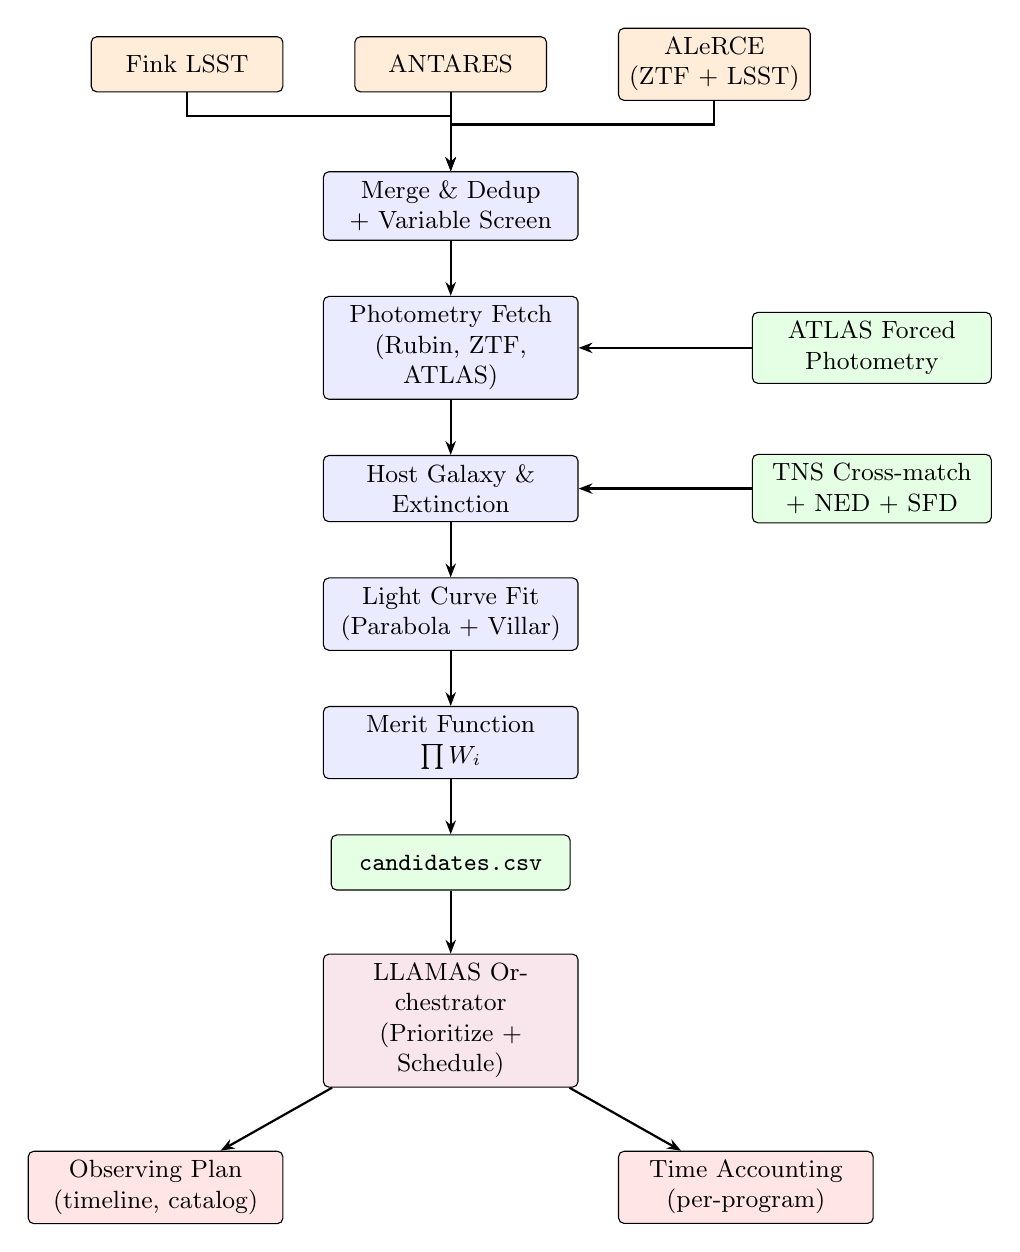
\begin{tikzpicture}[
    node distance=0.7cm and 0.9cm,
    block/.style={rectangle, draw, fill=blue!8, text width=3.0cm,
                  minimum height=0.8cm, align=center, rounded corners=2pt,
                  font=\small},
    broker/.style={rectangle, draw, fill=orange!15, text width=2.2cm,
                   minimum height=0.7cm, align=center, rounded corners=2pt,
                   font=\small},
    data/.style={rectangle, draw, fill=green!10, text width=2.8cm,
                 minimum height=0.7cm, align=center, rounded corners=2pt,
                 font=\small},
    output/.style={rectangle, draw, fill=red!10, text width=3.0cm,
                   minimum height=0.8cm, align=center, rounded corners=2pt,
                   font=\small},
    orch/.style={rectangle, draw, fill=purple!10, text width=3.0cm,
                 minimum height=0.8cm, align=center, rounded corners=2pt,
                 font=\small},
    arrow/.style={-{Stealth[length=5pt]}, thick},
]

% Brokers
\node[broker] (fink) {Fink LSST};
\node[broker, right=of fink] (antares) {ANTARES};
\node[broker, right=of antares] (alerce) {ALeRCE\\(ZTF + LSST)};

% Merge
\node[block, below=1.0cm of antares] (merge) {Merge \& Dedup\\+ Variable Screen};

% Enrichment
\node[block, below=of merge] (enrich) {Photometry Fetch\\(Rubin, ZTF, ATLAS)};

% Host & extinction
\node[block, below=of enrich] (host) {Host Galaxy \&\\Extinction};

% Fitting
\node[block, below=of host] (fit) {Light Curve Fit\\(Parabola + Villar)};

% Merit
\node[block, below=of fit] (merit) {Merit Function\\$\prod W_i$};

% candidates.csv
\node[data, below=of merit] (csv) {\texttt{candidates.csv}};

% Enrichment sources
\node[data, right=2.2cm of enrich] (atlas) {ATLAS Forced\\Photometry};
\node[data, right=2.2cm of host] (tns) {TNS Cross-match\\+ NED + SFD};

% Orchestrator
\node[orch, below=0.8cm of csv] (orch) {LLAMAS Orchestrator\\(Prioritize + Schedule)};

% Outputs
\node[output, below left=0.8cm and 0.5cm of orch] (plan) {Observing Plan\\(timeline, catalog)};
\node[output, below right=0.8cm and 0.5cm of orch] (acct) {Time Accounting\\(per-program)};

% Arrows
\draw[arrow] (fink.south) -- ++(0,-0.3) -| (merge.north);
\draw[arrow] (antares.south) -- (merge.north);
\draw[arrow] (alerce.south) -- ++(0,-0.3) -| (merge.north);
\draw[arrow] (merge) -- (enrich);
\draw[arrow] (enrich) -- (host);
\draw[arrow] (host) -- (fit);
\draw[arrow] (fit) -- (merit);
\draw[arrow] (merit) -- (csv);
\draw[arrow] (csv) -- (orch);
\draw[arrow] (orch) -- (plan);
\draw[arrow] (orch) -- (acct);
\draw[arrow] (atlas) -- (enrich);
\draw[arrow] (tns) -- (host);

\end{tikzpicture}
\caption{System data flow.  Five alert brokers feed into a cross-matching
and deduplication stage.  Photometry is fetched from Rubin (via Fink),
ZTF (via ALeRCE), and ATLAS.  Host galaxy classification, TNS
cross-matching, NED redshifts, and galactic extinction corrections are
applied.  Light curves are fit using inverted parabola and Villar SPM
models.  A six-component multiplicative merit function produces ranked
\texttt{candidates.csv}, which feeds into the LLAMAS orchestrator for
scheduling with time accounting.}
\label{fig:pipeline}
\end{figure}


\subsection{Code Organization}

\begin{center}
\small
\begin{tabular}{ll}
\toprule
Module & Purpose \\
\midrule
\multicolumn{2}{l}{\textit{Alert Pipeline}} \\
\texttt{run\_tonight.py} & Nightly CLI: all brokers $\to$ candidates.csv \\
\texttt{supernova\_monitor.py} & Multi-broker orchestrator class \\
\texttt{config.py} & Centralized configuration (merit weights, thresholds) \\
\texttt{core/alert\_aggregator.py} & Cross-match, deduplicate, merge \\
\texttt{core/peak\_fitting.py} & Peak fitting (parabola + Villar SPM + SALT2) \\
\texttt{core/magellan\_planning.py} & Merit function, observability, TCS catalog \\
\texttt{core/variable\_screen.py} & Known variable rejection (13.7k sources) \\
\texttt{core/report.py} & PDF report generation \\
\texttt{core/ddf\_fields.py} & DDF field definitions \\
\texttt{broker\_clients/fink\_client.py} & Fink LSST API (primary Rubin photometry) \\
\texttt{broker\_clients/antares\_client.py} & ANTARES cone search (parallel) \\
\texttt{broker\_clients/alerce\_client.py} & ALeRCE REST API (ZTF + LSST) \\
\texttt{broker\_clients/alerce\_db\_client.py} & ALeRCE direct PostgreSQL \\
\texttt{broker\_clients/atlas\_client.py} & ATLAS forced photometry (retry/backoff) \\
\texttt{broker\_clients/tns\_client.py} & TNS cross-match for duplicate detection \\
\texttt{broker\_clients/rubin\_tap\_client.py} & Rubin Science Platform TAP \\
\texttt{host\_galaxy/morphology\_filter.py} & Galaxy classification, nuclear offset \\
\texttt{utils/extinction.py} & Galactic extinction (IRSA SFD) \\
\texttt{utils/ned\_query.py} & NED redshift lookups \\
\texttt{cache/alert\_cache.py} & SQLite caching layer \\
\midrule
\multicolumn{2}{l}{\textit{LLAMAS Orchestrator}} \\
\texttt{orchestrator/config.py} & LLAMAS instrument config (LCO site, overhead) \\
\texttt{orchestrator/models.py} & Target, ScheduledEntry, ProgramAllocation, ObsPlan \\
\texttt{orchestrator/normalize.py} & Input loading, exposure estimation \\
\texttt{orchestrator/planner.py} & Twilight, observability, greedy scheduler \\
\texttt{orchestrator/prioritizer.py} & Composite priority scoring \\
\texttt{orchestrator/accounting.py} & Multi-program time tracking \\
\texttt{orchestrator/run\_nightly.py} & End-to-end nightly orchestration \\
\texttt{orchestrator/output.py} & Timeline, catalog, summary writers \\
\texttt{orchestrator/reporting.py} & Time reports, season progress \\
\texttt{orchestrator/cli.py} & CLI (plan, run-nightly, reconcile) \\
\bottomrule
\end{tabular}
\end{center}


%% =========================================================================
\section{Data Sources}
\label{sec:data_sources}
%% =========================================================================

The pipeline queries five independent alert broker and enrichment
sources, each providing different coverage, classifiers, and data
products.

\subsection{Fink LSST}

Fink\footnote{\url{https://fink-portal.org/}} processes Rubin/LSST
alerts through multiple ML classifiers including
\texttt{snnSnVsOthers} (SN vs.\ non-SN) and \texttt{earlySNIa} (early
Type~Ia identification).  The pipeline queries for candidates tagged as
\texttt{sn\_near\_galaxy\_candidate} and
\texttt{extragalactic\_new\_candidate}.  Fink serves as the primary
source of Rubin prompt photometry: multi-band ($grizy$) light curves
including DiaSource detections and forced photometry in nanoJanskys.

\subsection{ANTARES}

ANTARES\footnote{\url{https://antares.noirlab.edu/}} ingests both ZTF
and Rubin alert streams.  The pipeline performs cone searches of each
DDF field and filters for supernova-related tags.  ANTARES does not
provide a trained SN~Ia classifier; the pipeline computes a heuristic
proxy $P(\mathrm{Ia})$ \textbf{capped at 0.50} to prevent
ANTARES-only detections from dominating the ranking.

\subsection{ALeRCE (ZTF and LSST)}

ALeRCE\footnote{\url{https://alerce.online/}} processes both ZTF
alerts (random-forest classifier
\texttt{lc\_classifier\_BHRF\_forced\_phot}) and Rubin/LSST alerts
(stamp classifier \texttt{stamp\_classifier\_rubin}).  The ZTF
classifier provides per-class probabilities (SN~Ia, SN~II, SN~Ib/c,
SLSN); the LSST classifier distinguishes SN from AGN/variable/asteroid
but does not sub-classify SN types.  Direct PostgreSQL access provides
faster bulk queries than the REST API.

\subsection{ATLAS}

ATLAS\footnote{\url{https://fallingstar-data.com/forcedphot/}} provides
forced photometry in cyan ($c$) and orange ($o$) filters as an
enrichment source (not a primary classifier).  The pipeline uses batch
submission via the \texttt{radeclist} API with retry/backoff logic and
automatic token re-authentication on expiry.

\subsection{TNS}

The Transient Name Server\footnote{\url{https://www.wis-tns.org/}}
(TNS) is cross-matched at 5\arcsec\ radius to identify
already-reported candidates, retrieve IAU designations, and pull
existing spectroscopic classifications and redshifts.

\begin{table}[h]
\centering
\caption{Summary of alert broker and enrichment source properties.}
\label{tab:brokers}
\begin{tabular}{lcccl}
\toprule
Source & Survey & Role & Classifier & Notes \\
\midrule
Fink          & Rubin   & Primary  & ML (SN vs.\ other) & Full Rubin photometry \\
ANTARES       & ZTF+Rubin & Primary & Heuristic proxy & Capped at $P=0.50$ \\
ALeRCE (ZTF)  & ZTF     & Primary  & RF stamp classifier & $P(\mathrm{Ia})$ direct \\
ALeRCE (LSST) & Rubin   & Primary  & Stamp classifier & $P(\mathrm{SN})$ only \\
ATLAS         & ATLAS   & Enrichment & None & Forced photometry \\
TNS           & IAU     & Cross-match & None & Duplicate detection \\
\bottomrule
\end{tabular}
\end{table}


%% =========================================================================
\section{Alert Aggregation}
\label{sec:aggregation}
%% =========================================================================

The \texttt{AlertAggregator} class merges detections from all brokers
into a single, deduplicated candidate list.

\subsection{Cross-Matching and Deduplication}

Objects from different brokers are matched by coordinate proximity
($\leq 1\arcsec$) or shared ZTF \texttt{object\_id}.  For each unique
source, the pipeline retains broker-specific identifiers and
classification probabilities.

\subsection{Probability Normalization}

Each broker's classification probability is normalized to a common
$P(\mathrm{Ia})$ scale.  ALeRCE ZTF provides direct ML probability;
ALeRCE LSST uses $P(\mathrm{SN})$ as proxy; ANTARES uses a heuristic
capped at 0.50; Fink provides both \texttt{snnSnVsOthers} and
\texttt{earlySNIa} scores.

\subsection{Variable Star Screening}

The \texttt{VariableScreener} class cross-matches candidates against
13{,}749 known variable stars from Gaia~DR3 and VSX across the DDFs
(2\arcsec\ matching radius).

\subsection{TNS Cross-Match}

Candidates are cross-matched against TNS at 5\arcsec\ to identify
already-reported transients, retrieve IAU designations (AT/SN names),
spectroscopic classifications, and redshifts.  This prevents duplicate
follow-up of known objects.

\subsection{Nuclear Offset Filter}

Using host galaxy positions from GLADE+, SDSS, PS1, and SkyMapper, the
pipeline computes the angular offset between each transient and its host
nucleus.  Candidates with offset $< 1\arcsec$ are flagged as likely
AGN or TDE (nuclear transients); offsets of 1--30\arcsec\ are consistent
with SNe in host galaxies.


%% =========================================================================
\section{Light Curve Peak Fitting}
\label{sec:peak_fitting}
%% =========================================================================

The \texttt{core/peak\_fitting.py} module estimates peak brightness
and timing using a dual-fit strategy for robustness.

\subsection{Inverted Parabola Model}

Near maximum light, the flux light curve is approximately parabolic:
\begin{equation}
f(t) = f_{\mathrm{peak}} - a\,(t - t_0)^2,
\end{equation}
fit independently per band using \texttt{scipy.optimize.curve\_fit}
with flux uncertainties as weights.

\subsection{Multi-Band Villar SPM}
\label{sec:villar}

The primary method fits the Villar supernova parametric model
\citep{Villar2019} simultaneously across all bands with a shared
explosion epoch $t_0$:
\begin{equation}
F(t) =
\begin{cases}
\displaystyle
\frac{A\!\left[1 - \beta\,\frac{t - t_0}{t_0 + \gamma - t_0}\right]}
{1 + \exp\!\left(-\frac{t - t_0}{\tau_{\mathrm{rise}}}\right)},
& t < t_0 + \gamma, \\[12pt]
\displaystyle
\frac{A(1-\beta)\,\exp\!\left(-\frac{t - t_0 - \gamma}{\tau_{\mathrm{fall}}}\right)}
{1 + \exp\!\left(-\frac{t - t_0}{\tau_{\mathrm{rise}}}\right)},
& t \geq t_0 + \gamma,
\end{cases}
\end{equation}
with $1 + 5N_b$ parameters for $N_b$ bands.  Peak time is determined
by numerical flux maximization on a fine grid rather than the analytic
approximation.

\subsection{Multi-Survey Photometry Combination}

The pipeline combines photometry from up to three surveys before
fitting: Rubin/LSST (via Fink, $grizy$, nJy), ZTF (via ALeRCE,
$gr$), and ATLAS (forced photometry, cyan/orange).  All flux is
standardized to nanoJanskys.

\subsection{Optional SALT2 Template Fitting}

If \texttt{sncosmo} is installed, a SALT2 template fit provides
stretch ($x_1$), color ($c$), and rest-frame $B$-band peak magnitude.


%% =========================================================================
\section{Merit Function}
\label{sec:merit}
%% =========================================================================

The alert pipeline computes a six-component multiplicative merit
function encoding the scientific value of spectroscopically observing
each candidate:
\begin{equation}
\label{eq:merit}
\boxed{\mathcal{M} = W_{\mathrm{time}} \times W_{\mathrm{mag}}
\times W_{\mathrm{prob}} \times W_{\mathrm{host}} \times
W_{\mathrm{ext}} \times W_{\mathrm{broker}}}
\end{equation}

\begin{center}
\begin{tabular}{lll}
\toprule
Component & Formula & Default Parameters \\
\midrule
$W_{\mathrm{time}}$ & $\exp(-\Delta t^2 / 2\tau^2)$ &
  $\tau = 10$ days \\
$W_{\mathrm{mag}}$ & $\exp(-(m - m_{\mathrm{opt}})^2 / \sigma_m^2)$ &
  $m_{\mathrm{opt}} = 20.5$, $\sigma_m = 1.25$ \\
$W_{\mathrm{prob}}$ & $P(\mathrm{Ia}) \in [0.1, 1.0]$ &
  Clipped lower bound \\
$W_{\mathrm{host}}$ & $\{1.0, 0.6, 0.7\}$ &
  Elliptical, Spiral, Unknown \\
$W_{\mathrm{ext}}$ & $\exp(-E(B\!-\!V) / 0.15)$ &
  Penalizes high extinction \\
$W_{\mathrm{broker}}$ & $1.0 + 0.1 \times (N - 1)$ &
  Multi-broker agreement \\
\bottomrule
\end{tabular}
\end{center}

The multiplicative structure ensures a candidate must score well on
\emph{all} factors.  A single high score (e.g., bright magnitude) cannot
compensate for a poor score elsewhere (e.g., far past peak).


%% =========================================================================
\section{LLAMAS Orchestrator}
\label{sec:orchestrator}
%% =========================================================================

The LLAMAS orchestrator converts ranked \texttt{candidates.csv} output
from the alert pipeline into executable observing plans for the MAGNETS
collaboration.

\subsection{Exposure Estimation}

Exposure times are estimated using a three-tier cascade from the Stubbs
2026B proposal Table~1:

\begin{center}
\begin{tabular}{lccc}
\toprule
Strategy & Input & Example & Fallback \\
\midrule
Redshift table & $z$ known & $z = 0.25 \to 95$~min (grey) & --- \\
Magnitude scaling & mag known & mag~20 $\to$ 45~min, $2.5\times$/mag & --- \\
Default & neither & 45~min & Always \\
\bottomrule
\end{tabular}
\end{center}

The redshift-based table encodes moon phase constraints:
\begin{center}
\begin{tabular}{cccc}
\toprule
$z$ range & Moon phase & Peak $r$ & Exposure \\
\midrule
0.10--0.20 & Bright & 19.3 & 35~min \\
0.20--0.30 & Grey & 20.6 & 95~min \\
0.30--0.35 & Grey/Dark & 21.3 & 100~min \\
0.35--0.40 & Dark & 21.9 & 180~min \\
\bottomrule
\end{tabular}
\end{center}

\subsection{Composite Priority Scoring}

The orchestrator's prioritizer computes a composite score incorporating
multiple signals:
\begin{equation}
S = \underbrace{W_{\mathrm{sci}} \times 100}_{\text{science}}
\times \underbrace{F_{\mathrm{budget}}}_{\text{time budget}}
\times \underbrace{W_{\phi}}_{\text{LC phase}}
+ \underbrace{f_{\mathrm{obs}} \times 20}_{\text{observability}}
+ \underbrace{\Delta_{\mathrm{kw}} \times 50}_{\text{keywords}}
\end{equation}
where:
\begin{itemize}
\item $W_{\mathrm{sci}}$: P1$\to$1.0, P2$\to$0.7, P3$\to$0.4, P4$\to$0.2
\item $F_{\mathrm{budget}}$: 1.0 ($>$5h remaining), 0.5 (0--5h), 0.1 (exhausted)
\item $W_\phi$: phase weight from alert pipeline ($W_{\mathrm{time}} = \exp(-\Delta t^2/2\tau^2)$)
\item $f_{\mathrm{obs}}$: fraction of night target is above airmass limit
\item $\Delta_{\mathrm{kw}}$: keyword adjustments (``HIGH PRIORITY'' $+0.3$, ``backup'' $-0.3$)
\end{itemize}

The phase weight $W_\phi$ ensures targets near peak brightness are
automatically prioritized over those well past peak, even at the same
nominal priority level.

\subsection{Greedy Scheduling Algorithm}

Targets are scheduled using a greedy algorithm adapted from existing
LDSS3 scheduling tools:
\begin{equation}
\mathrm{score}_i(t) = S_i - \alpha(t) \times 10
\end{equation}
where $S_i$ is the composite priority and $\alpha(t)$ is the airmass
at time~$t$.  At each time step, the highest-scoring observable target
is scheduled.  Spectrophotometric standard stars from the Boyd et al.\
WD catalog are interleaved at the start and end of the night.

Key parameters: maximum airmass 1.6, IFU overhead 1~min, gap fill up
to 5~min, sub-exposures capped at 900~s.

\subsection{Multi-Program Time Accounting}

Time is tracked per program per moon phase using an \texttt{allocations.yaml}
configuration:

\begin{lstlisting}[language={}]
semester: "2026B"
default_program: "MAGNETS-Stubbs"
programs:
  - program: "MAGNETS-Stubbs"
    pi: "Stubbs"
    allocated_hours: {dark: 5.0, grey: 20.0, bright: 5.0}
  - program: "MAGNETS-Villar"
    pi: "Villar"
    allocated_hours: {dark: 4.0, grey: 8.0, bright: 4.0}
\end{lstlisting}

Time is charged when plans are generated (charge-on-schedule), with a
\texttt{reconcile} command for post-night adjustment.  State is
persisted in \texttt{time\_accounting.json} with a full charge log for
audit.

\subsection{Outputs}

The orchestrator produces:
\begin{itemize}
\item \textbf{Timeline}: UT schedule with standard stars, exposure
parameters, and priority annotations
\item \textbf{TCS catalog}: Magellan telescope control system format
(16-field, J2000)
\item \textbf{Summary}: Human-readable plan with efficiency metrics and
per-program time budget status
\item \textbf{Time report}: Per-program charges and remaining budget
\item \textbf{Season report}: Cumulative usage, burn rate, projected
exhaustion
\end{itemize}


%% =========================================================================
\section{Galactic Extinction and Host Galaxy}
\label{sec:environment}
%% =========================================================================

\subsection{Extinction Corrections}

The pipeline queries the IRSA Galactic Dust Reddening service using the
\citet{Schlafly2011} recalibration of the \citet{Schlegel1998} (SFD)
dust map.  Extinction values $A_\lambda$ for SDSS $ugriz$ are cached in
SQLite.  The $E(B\!-\!V)$ reddening is computed from $A_g / R_g$ with
$R_g = 3.303$.

\subsection{Host Galaxy Classification}

The \texttt{MorphologyFilter} queries SDSS, Pan-STARRS, SkyMapper, and
GLADE+ (22M galaxies) for host galaxy morphology using optical color
cuts ($g-r > 0.55$ and $r-i > 0.15$ for ellipticals).  NED provides
spectroscopic redshifts for distance modulus computation.


%% =========================================================================
\section{Current Status}
\label{sec:status}
%% =========================================================================

\subsection{Implemented}

\paragraph{Alert Pipeline:}
\begin{itemize}
\item Five-broker alert ingestion (Fink, ANTARES, ALeRCE-ZTF,
ALeRCE-LSST, ATLAS) with DDF-targeted queries
\item TNS cross-matching for duplicate detection and IAU designations
\item Cross-matching and deduplication (1\arcsec\ tolerance + shared ZTF IDs)
\item Variable star screening (13{,}749 sources from Gaia~DR3/VSX)
\item Nuclear offset filter for AGN/TDE rejection
\item Galactic extinction corrections (IRSA SFD) with SQLite caching
\item NED spectroscopic redshifts and distance moduli
\item Host galaxy morphology (SDSS/PS1/SkyMapper/GLADE+)
\item Multi-band light curve fitting (parabola + Villar SPM + optional SALT2)
\item Multi-survey photometry combination (Rubin + ZTF + ATLAS)
\item Six-component multiplicative merit function
\item Rise time constraints filter ($>$30~day risers rejected)
\item ZTF batch photometry via ALeRCE direct PostgreSQL
\item ATLAS forced photometry with retry/backoff and token re-auth
\item PDF report generation with merit breakdowns, sky maps, light curves
\item Slew-minimized observing sequence optimization
\item SQLite caching across all external queries
\end{itemize}

\paragraph{LLAMAS Orchestrator:}
\begin{itemize}
\item Exposure estimation cascade (redshift table $\to$ magnitude $\to$ fallback)
\item Greedy scheduling with composite priority scoring
\item Phase-aware prioritization ($W_\phi$ from alert pipeline)
\item Multi-program time accounting (charge-on-schedule + reconciliation)
\item WD spectrophotometric standard star interleaving
\item CLI with three subcommands (\texttt{plan}, \texttt{run-nightly},
\texttt{reconcile})
\item Nightly time reports and season progress reporting
\item Magellan TCS catalog output
\end{itemize}

\subsection{Remaining Work}

\begin{itemize}
\item Integration test with real alert pipeline \texttt{candidates.csv}
\item Historical validation on archived DP1 data
\item Unit tests with pytest coverage
\item Boyd et al.\ 2026 WD standard catalog integration
\item Google Sheet ingester for manual target requests
\item Multi-night look-ahead optimization
\end{itemize}


%% =========================================================================
\section*{References}
%% =========================================================================

\begin{thebibliography}{9}

\bibitem[Schlegel et al.(1998)]{Schlegel1998}
Schlegel, D.~J., Finkbeiner, D.~P., \& Davis, M.\ 1998,
\textit{ApJ}, 500, 525.

\bibitem[Schlafly \& Finkbeiner(2011)]{Schlafly2011}
Schlafly, E.~F., \& Finkbeiner, D.~P.\ 2011,
\textit{ApJ}, 737, 103.

\bibitem[Villar et al.(2019)]{Villar2019}
Villar, V.~A., et al.\ 2019,
\textit{ApJ}, 884, 83.

\end{thebibliography}


\end{document}
